%
\subsection{Remote server}
\label{sec:remote-serv-decomp}
In this section the remote server is analyzed, considering its events, use
cases, dynamic operation and the flow of events.

\subsubsection{User mock-ups}
\label{sec:user-mockups-2}
Fig.~\ref{fig:user-mockups-rs} illustrates the user mock-ups for the
\texttt{Remote Server}. It intends to mimic the user interaction with the
\texttt{Remote server} interface,
clarifying the user actions and the respective responses, as well as the
workflow, defining the \texttt{Remote Server} interface.
%
\begin{figure}[htb!]
\centering
    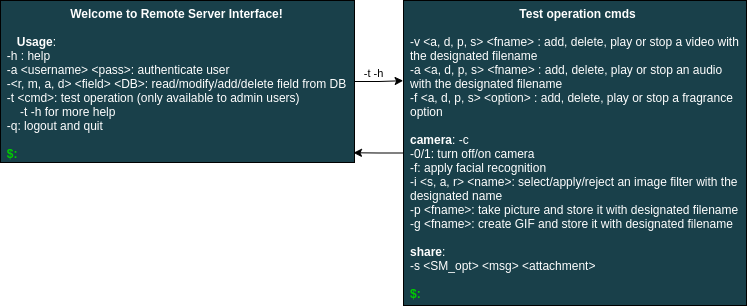
\includegraphics[width=1.0\columnwidth]{./img/user-mockups-rs.png}
  \caption{User mock-ups: Remote Server}%
\label{fig:user-mockups-rs}
\end{figure}

It consists of a \gls{cli} providing basic commands to authenticate an user,
perform operations over a \gls{db} and test the operation of a designated
\texttt{Local System} (only available to administrator users).

To test the operation of a \texttt{Local System}, an \texttt{Admin} can:
\begin{item-c}
\item \emph{Normal mode}: add, delete, play or stop video, audio and fragrance;
\item \emph{Interactive\& Multimedia modes} --- camera: turn on/off the camera, apply facial
  recognition, use an image filter, take a picture or create a \gls{gif};
\item \emph{Sharing mode}: share to a designated social media network a post,
  containing a message and attachment (picture or \gls{gif}). 
\end{item-c}
%
%The initial state of the \gls{mdo-l}'s~\gls{ui} is depicted in thick border
%outline, after a \texttt{User} has been detected --- \texttt{Interaction
%  mode}. On the left it is the camera feed and on the right the commands ribbon,
%containing the hints to use the system and the available options. As it can
%been, the \texttt{User} can choose an option by hovering with pointing finger
%over the desired option for a designated amount of time (e.g., 3 seconds).
%
%The workflow can be as follows:
%\begin{item-c}
%\item If the \texttt{User} selects the \texttt{Image filter} option, the
%  \texttt{Image filtering} view is shown, presenting the options to select
%  filters (which can be scrolled through palm raising/lowering), to cancel or
%  accept the image filter. If a filter is selected \texttt{filter1\_pressed}, it
%  is applied, and if accepted it will return to \texttt{Interaction mode},
%  keeping the filter on.
%\item If the \texttt{User} selects the \texttt{Take Pic} option, \texttt{Picture
%  mode} is started with a timer to allow the \texttt{User} to get ready before
%actually taking the picture. The \texttt{User} can \texttt{Cancel} --- returning
%to main menu --- or \texttt{Share} --- starting \texttt{Sharing mode}.
%\item If the \texttt{User} selects the \texttt{Create GIF} option, \texttt{GIF
%    mode (setup)} is started with a timer to allow the \texttt{User} to get
%  ready before actually creating the \gls{gif}. After the \texttt{setup\_timer}
%  is elapsed, the \texttt{GIF mode (operation)} starts, displaying a dial with
%  the \gls{gif} duration until being complete. When the \texttt{gif\_timer}
%  elapses, the \gls{gif} is created, enabling the \texttt{User} to
%  \texttt{Cancel} --- returning to main menu --- or to \texttt{Share} ---
%  starting \texttt{Sharing mode}.
%\item Lastly, in the \texttt{Sharing mode}, the \texttt{User} can
%  \texttt{Cancel} --- returning to main menu --- or select the
%  social media network. After selecting the social media, the \texttt{User} can
%  edit the post by entering its customized message and, if \texttt{Share} is
%  pressed, a message box will appear displaying the status of the post sharing
%  --- \texttt{Success} or \texttt{Error}.
%\end{item-c}
%

\subsubsection{Events}
\label{sec:events-2}
%
Table~\ref{tab:events-rs} presents the most relevant events for the
\texttt{Remote Server}, categorizing them by their source and synchrony and
linking it to the system's intended response.

\begingroup
\renewcommand{\arraystretch}{0.7} % Default value: 1
% Please add the following required packages to your document preamble:
% \usepackage{booktabs}
\begin{table}[hbt!]
\centering
\caption{Events: Remote Server}
\label{tab:events-rs}
\begin{tabular}{@{}llll@{}}
\toprule
\textbf{Event}          & \textbf{System response}                                                                                                     & \textbf{Source}                                                 & \textbf{Type} \\ \midrule
Power on                & Initialize RDBMS and go to Idle mode                                                                                         & System maintainer                                               & Asynchronous  \\ \midrule
Connection Requested    & Accept/refuse connection                                                                                                     & Remote Client                                                   & Asynchronous  \\ \midrule
Connection Accepted     & Start listening for commands                                                                                                 & Remote Client                                                   & Asynchronous  \\ \midrule
Authenticate            & \begin{tabular}[c]{@{}l@{}}Query User DB to validate user credentials.\\ If valid, login user.\end{tabular}                  & Remote Client                                                   & Asynchronous  \\ \midrule
Help                    & Send help information                                                                                                        & Remote Client                                                   & Asynchronous  \\ \midrule
Logout                  & \begin{tabular}[c]{@{}l@{}}Logout user, close connection and go to\\ Idle mode\end{tabular}                                  & Remote Client                                                   & Asynchronous  \\ \midrule
Check WiFi connection   & Periodically check WiFi connection                                                                                           & Remote Client                                                   & Synchronous   \\ \midrule
Connection timeout      & \begin{tabular}[c]{@{}l@{}}Logout user, close connection and go to \\ Idle mode\end{tabular}                                 & Remote Server                                                   & Synchronous   \\ \midrule
DB management           & Read/modify/add/delete data from DB                                                                                          & Remote Client                                                   & Asynchronous  \\ \midrule
Update stations         & Update all ready-to-run stations with ads data                                                                               & Remote Server                                                   & Synchronous   \\ \midrule
Command invalid         & Inform RC that command is invalid                                                                                            & Remote Server                                                   & Synchronous   \\ \midrule
Station notification    & Store station notification into DB                                                                                           & Local System                                                    & Asynchronous  \\ \midrule
Test Operation RC       & \begin{tabular}[c]{@{}l@{}}Parse command originated from RC and, if valid, \\ dispatch it to designated station\end{tabular} & \begin{tabular}[c]{@{}l@{}}Remote Client\\ (Admin)\end{tabular} & Asynchronous  \\ \midrule
Test Operation Callback & Provide command dispatch to original RC                                                                                      & Local System                                                    & Asynchronous  \\ \bottomrule
\end{tabular}
\end{table}

\subsubsection{Use cases}
\label{sec:use-cases-2}

Fig.~\ref{fig:use-cases-rs} depicts the use cases diagram for the \texttt{Remote Server}, describing how the system should respond under various conditions to a request from one of the stakeholders to deliver a specific
goal.

\begin{figure}[htb!]
\centering
    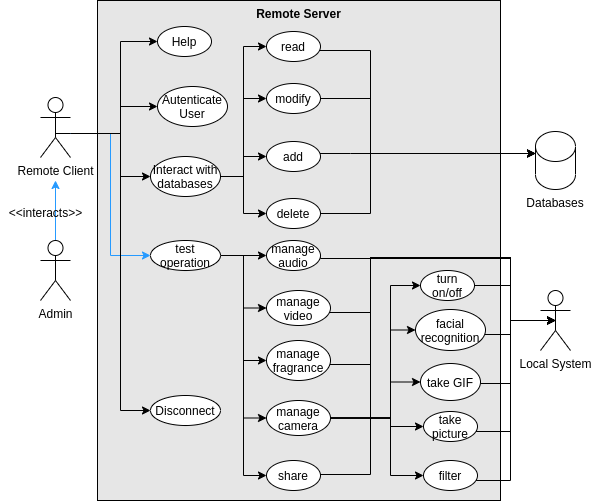
\includegraphics[width=0.6\columnwidth]{./img/use-cases-rs.png}
  \caption{Use cases: remote server}%
\label{fig:use-cases-rs}
\end{figure}

As it can be seen, the \texttt{Remote Client} can interact through various modes: \texttt{Help}, \texttt{Authenticate User}, \texttt{Interact with databases}, \texttt{Test Operation} and \texttt{Disconnect}.
When interacting with the databases, it is possible to read, modify, add or delete some field from a \texttt{Database}.
When testing the operation of the \texttt{Local System}, it is possible to \texttt{manage audio, video, fragrance and camera} and it is also possible to test the \texttt{share} option.
Between the \texttt{Manage Camera} option, there is \texttt{Turn On/Off, facial recognition, take GIF, take picture} and \texttt{filter}.
Note that only the \texttt{Admin} can use the \texttt{Test Operation}.

\subsubsection{Dynamic operation}
\label{sec:dyn-oper-2}
Fig.~\ref{fig:state-mach-rs} depicts the state machine diagram for the
\texttt{Local System}, illustrating its dynamic behavior. There are two main
states:
\begin{item-c}
\item \emph{\texttt{Initialization}}: the \texttt{Remote Server} is initialized. The settings are
  and \gls{db}s are loaded and if invalid they are restored. The WiFi
  communication is setup, signaling the communication status and if valid, an
  \gls{ip} address is returned. Lastly, the \gls{rdbms} is configured and started: if any error
  occurs the device goes into the \texttt{Critical Error} state, dumping the
  error to a log file and waiting for reset; otherwise, the initialization is
  complete.
\item \emph{\texttt{Execution}}: after the initialization is successful, the
  system goes into the \texttt{Execution} macro composite state with several
  concurrent activities, modeled as composite states too. However, it should be
  noted that there is only one actual state for the device, although at the
  perceivable time scale they appear to happen simultaneously. These activities
  are communication management (\texttt{Comm Manager}), \gls{db} management
  (\texttt{DB manager}), and request handling (\texttt{Request Handler}), and
  are executed forever until system's power off. They are detailed next.
\end{item-c}
%
\begin{figure}[htb!]
\centering
    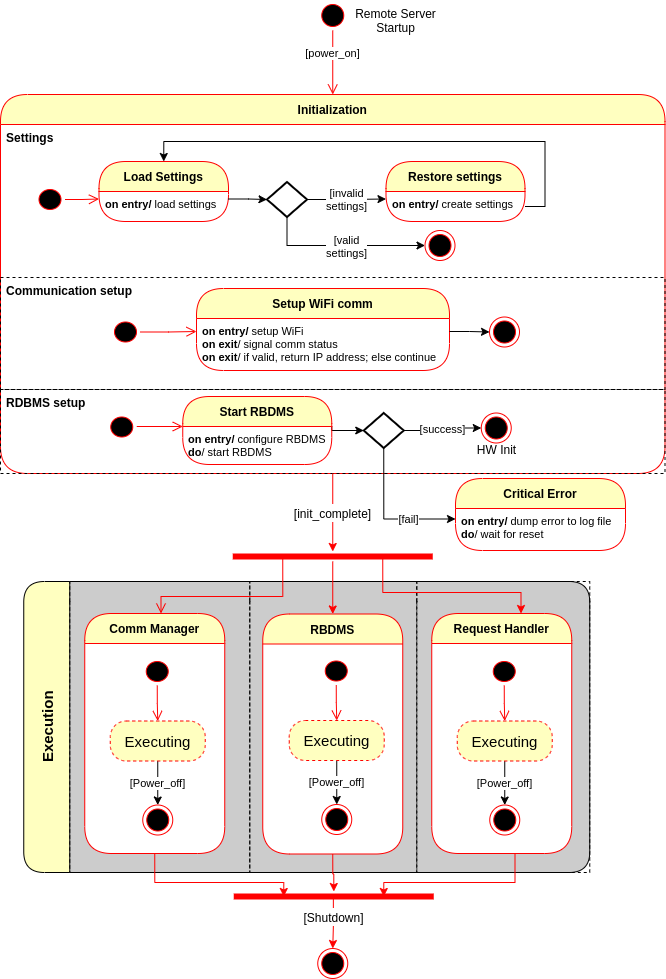
\includegraphics[width=0.7\columnwidth]{./img/state-mach-rs.png}
  \caption{State machine diagram: Remote server}%
\label{fig:state-mach-rs}
\end{figure}
%
%
\paragraph{\emph{Communication Manager}}
Fig.~\ref{fig:state-mach-rs-comm} depicts the state machine diagram for the
\texttt{Comm Manager} component. Upon successful initialization the
\texttt{Comm Manager} goes to \texttt{Idle}, listening for incoming
connections. When a remote node tries to connects, it makes a connection request
which can be accepted or denied. If the connection is accepted and the node
authenticates successfully the \texttt{Comm Manager} is ready for bidirectional
communication. When a message is received from the remote node, it is written to
\texttt{TX msg queue} and the \texttt{Request Handler} is notified. When a message
must be sent to the remote, it is read from the \texttt{TX msg queue} and sent
to the recipient. If the connection goes down, it is restarted, going into
\texttt{Idle} state again.
%
\begin{figure}[htb!]
\centering
    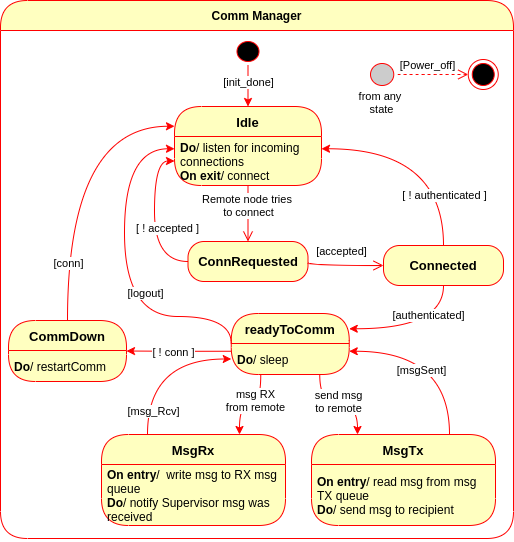
\includegraphics[width=0.6\columnwidth]{./img/state-mach-rs-comm.png}
  \caption{State machine diagram: Remote Server --- Comm Manager}%
\label{fig:state-mach-rs-comm}
\end{figure}
%
%
\paragraph{\emph{Database Manager}}
Fig.~\ref{fig:state-mach-rs-db} depicts the state machine diagram for the
\texttt{DB Manager} component. Upon successful initialization the
\texttt{DB Manager} goes to \texttt{Idle}, waiting for incoming \gls{db}
requests.
%
\begin{figure}[htb!]
\centering
    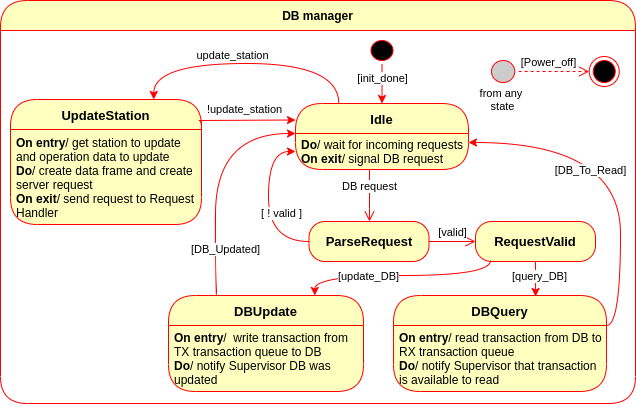
\includegraphics[width=0.7\columnwidth]{./img/state-mach-rs-db.png}
  \caption{State machine diagram: Remote Server --- \gls{db} Manager}%
\label{fig:state-mach-rs-db}
\end{figure}
%

When a request arrives, it is parsed, checking its validity. If the request is a
\gls{db} query, a transaction is read from the respective \gls{db} to the
\texttt{RX transaction queue} and the \texttt{Supervisor} is notified that there
is a transaction to read. Otherwise, if the request is a \gls{db} update
the transaction is written from the \texttt{TX transaction queue} to the
\gls{db} and the \texttt{Supervisor} is notified that the \gls{db} was updated.

Alternatively, the \gls{rdbms} can be triggered to update a station
(\texttt{update\_station} event), retrieving the station and operation data to
update. A data frame is composed and a server request is created, signaling it
to the \texttt{Request Handler} to process it.
%
\paragraph{\emph{Request Handler}}
Fig.~\ref{fig:state-mach-rs-req} depicts the state machine diagram for the
\texttt{Request Handler} component, which handles incoming requests from the
  \texttt{Remote Client}, \texttt{Local System}, or internally (to update stations). When a request arrives, it is parsed, and, if valid,
  the appropriate callback is triggered, processing the request and returning
  its output.
%  
\begin{figure}[htb!]
  \centering
  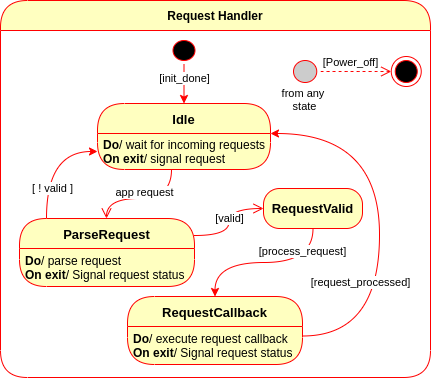
\includegraphics[width=0.55\textwidth]{img/state-mach-rs-req.png}%
  \caption{State machine diagram: Remote Server --- Request Handler}%
  \label{fig:state-mach-rs-req}
\end{figure}
  %
%
%

\subsubsection{Flow of events}
\label{sec:flow-events-2}

The flow of events throughout the system is described using a sequence diagram, comprising the interactions between the most relevant system's entities.
It is usually pictured as the visual representation of an use case. The main sequence diagrams are illustrated next.
%
%
\begin{figure}[htb!]
  \centering
  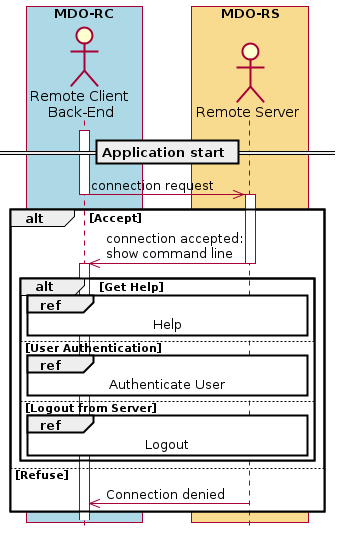
\includegraphics[width=0.4\textwidth]{img/seq-rs-general.png}%
  \caption{Sequence diagram: Remote Server}%
  \label{fig:seq-rs-general}
\end{figure}
%
\begin{figure}[htb!]
  \centering
  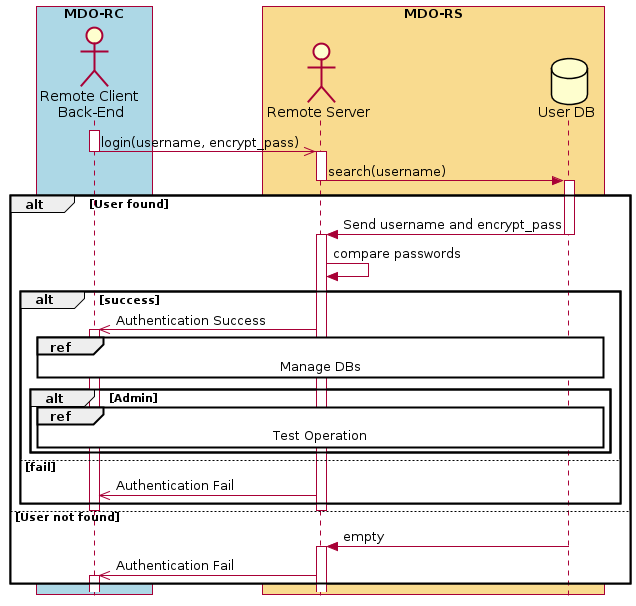
\includegraphics[width=0.55\textwidth]{img/seq-rs-authenticate.png}%
  \caption{Sequence diagram: Remote Server --- Authentication}%
  \label{fig:seq-rs-authenticate}
\end{figure}

\begin{figure}[htb!]
  \centering
  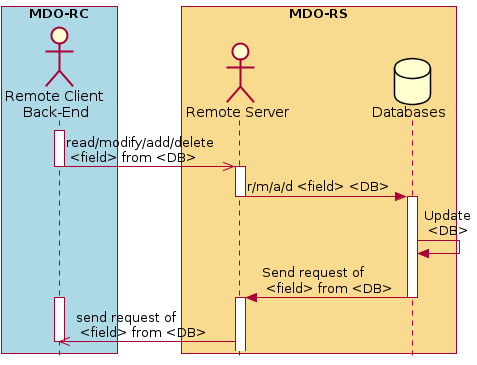
\includegraphics[width=0.55\textwidth]{img/seq-rs-manage-dbs.png}%
  \caption{Sequence diagram: Remote Server --- Manage Databases}%
  \label{fig:seq-rs-manage-dbs}
\end{figure}

\begin{figure}[htb!]
  \centering
  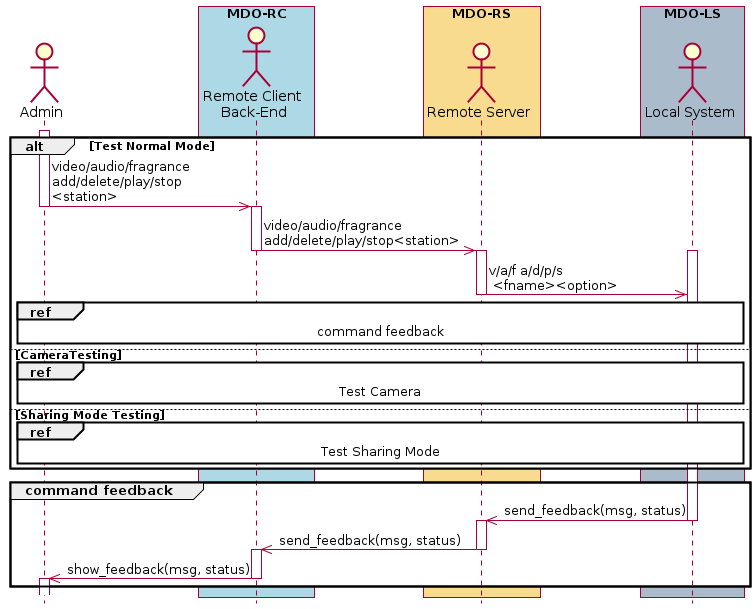
\includegraphics[width=0.8\textwidth]{img/seq-rs-test-op.png}%
  \caption{Sequence diagram: Remote Server --- Test Operation}%
  \label{fig:seq-rs-test-op}
\end{figure}

\begin{figure}[htb!]
  \centering
  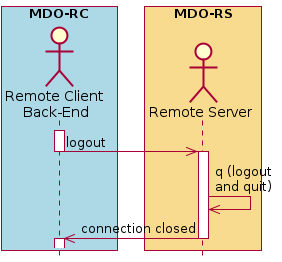
\includegraphics[width=0.4\textwidth]{img/seq-rs-logout.png}%
  \caption{Sequence diagram: Remote Server --- logout}%
  \label{fig:seq-rs-logout}
\end{figure}

The main interaction in all diagrams occurs between the \texttt{Remote Client} and the \texttt{Remote System}.

In first place, Fig.~\ref{fig:seq-rs-general} shows the \texttt{Application Start}, starting with a connection request that it can be either accepted or denied.

In second place, Fig.~\ref{fig:seq-rs-authenticate} shows the \texttt{Authentication} process, where the \texttt{Remote Client} sends the username and the password to the \texttt{Remote Server}.
This last search for the username in the \texttt{User DB}, if it is not found, the authentications fails, else, the \texttt{Remote Server} compares the passwords and Sends the authentication success or fail for the cases where the password is equal or not equal, respectively.
It is only possible to access the \texttt{Manage DBs} and the \texttt{Test Operation} if the authentication succeeds.

In Fig.~\ref{fig:seq-rs-manage-dbs} the \texttt{Remote Client} requests to interact with some field of some \texttt{Database} to \texttt{Remote Server}.
The \texttt{Remote Server} makes the request to the specific \texttt{Database}, receive the response and responds to the \texttt{Remote Client}.

In Fig.~\ref{fig:seq-rs-test-op} it can be seen the \texttt{Test Operation}.
As said previously, only the admin can access this part, where it can test the functionality of any \texttt{Local System}.
The \texttt{Admin} sends the request to the \texttt{Remote Client} that then sends it to the \texttt{Remote Server} with the specific station.
Then, the \texttt{Remote Server} interacts with the specific station, making the specific \texttt{Local System} acts according to the command that was sent.  
%%% Local Variables:
%%% mode: latex
%%% TeX-master: "../../../dissertation"
%%% End:
